\documentclass[a4paper,12pt]{book}
\usepackage[ascii]{inputenc}
\usepackage[T1]{fontenc}
\usepackage[french,english]{babel}
\usepackage{amsmath,amssymb,amsfonts,textcomp}
\usepackage{color}
\usepackage{calc}
\usepackage{longtable}
\usepackage{hyperref}
\usepackage{graphics}
\usepackage{graphicx}
\DeclareGraphicsExtensions{.jpg}
\DeclareGraphicsExtensions{.png}
\hypersetup{colorlinks=true, linkcolor=blue, filecolor=blue, pagecolor=blue, urlcolor=blue}

%%%%\%%%%%%%% titre, auteurs, date, etc...%%%%%%%%%%%%%%%%%%
\title{\Huge The CanFestival CANOpen stack manual}
\author{Edouard TISSERANT}
\date{\today}

% Text styles
%\newcommand\textstyleTeletype[1]{\texttt{#1}}
% Outline numbering
\setcounter{secnumdepth}{5}
\renewcommand\thesection{\arabic{section} -}
\renewcommand\thesubsection{\arabic{section}.\arabic{subsection})}
\renewcommand\thesubsubsection{\arabic{section}.\arabic{subsection}.\arabic{subsubsection})}
\renewcommand\theparagraph{\alph{paragraph})}
\renewcommand\thesubparagraph{\roman{subparagraph})}
% List styles
\newcommand\liststyleLi{%
\renewcommand\labelitemi{{--}}
\renewcommand\labelitemii{{--}}
\renewcommand\labelitemiii{{--}}
\renewcommand\labelitemiv{{--}}
}
\newcommand\liststyleLii{%
\renewcommand\labelitemi{{--}}
\renewcommand\labelitemii{{--}}
\renewcommand\labelitemiii{{--}}
\renewcommand\labelitemiv{{--}}
}
\newcommand\liststyleLiii{%
\renewcommand\labelitemi{{--}}
\renewcommand\labelitemii{{--}}
\renewcommand\labelitemiii{{--}}
\renewcommand\labelitemiv{{--}}
}
\newcommand\liststyleLiv{%
\renewcommand\labelitemi{{--}}
\renewcommand\labelitemii{{--}}
\renewcommand\labelitemiii{{--}}
\renewcommand\labelitemiv{{--}}
}
\newcommand\liststyleLv{%
\renewcommand\labelitemi{{--}}
\renewcommand\labelitemii{{--}}
\renewcommand\labelitemiii{{--}}
\renewcommand\labelitemiv{{--}}
}
\newcommand\liststyleLvi{%
\renewcommand\labelitemi{{--}}
\renewcommand\labelitemii{{--}}
\renewcommand\labelitemiii{{--}}
\renewcommand\labelitemiv{{--}}
}
\newcommand\liststyleLvii{%
\renewcommand\labelitemi{{--}}
\renewcommand\labelitemii{{--}}
\renewcommand\labelitemiii{{--}}
\renewcommand\labelitemiv{{--}}
}
\newcommand\liststyleLviii{%
\renewcommand\labelitemi{{--}}
\renewcommand\labelitemii{{--}}
\renewcommand\labelitemiii{{--}}
\renewcommand\labelitemiv{{--}}
}
\newcommand\liststyleLix{%
\renewcommand\labelitemi{{--}}
\renewcommand\labelitemii{{--}}
\renewcommand\labelitemiii{{--}}
\renewcommand\labelitemiv{{--}}
}
\newcommand\liststyleLx{%
\renewcommand\labelitemi{{--}}
\renewcommand\labelitemii{{--}}
\renewcommand\labelitemiii{{--}}
\renewcommand\labelitemiv{{--}}
}
\newcommand\liststyleLxi{%
\renewcommand\labelitemi{{--}}
\renewcommand\labelitemii{{--}}
\renewcommand\labelitemiii{{--}}
\renewcommand\labelitemiv{{--}}
}
\newcommand\liststyleLxii{%
\renewcommand\labelitemi{{--}}
\renewcommand\labelitemii{{--}}
\renewcommand\labelitemiii{{--}}
\renewcommand\labelitemiv{{--}}
}
\newcommand\liststyleLxiii{%
\renewcommand\labelitemi{{\textbullet}}
\renewcommand\labelitemii{{\textbullet}}
\renewcommand\labelitemiii{{\textbullet}}
\renewcommand\labelitemiv{{\textbullet}}
}

\begin{document}

{\centering\sffamily\Huge The CanFestival CANOpen stack manual.}

\renewcommand\contentsname{CanFestival v3.0 Manual}
\setcounter{tocdepth}{2}
\tableofcontents
\section{Introduction}
CanFestival is an OpenSource (LGPL and GPL) CANOpen framework.

\subsection{The CanFestival project}
This project, initiated by Edouard TISSERANT in 2001, as grown thanks to
Francis DUPIN and other contributors.

Today, CanFestival focuses on providing an ANSI{}-C platform independent
CANOpen stack that can be implemented as master or slave nodes on PCs,
Real{}-time IPCs, and Microcontrollers.

CanFestival is a project supported by Lolitech.

\subsection{What is CANopen}
CANopen is a CAN based high level protocol. It defines some protocols to
:

\liststyleLi
\begin{enumerate}
\item Configure a CAN network.
\item Transmit data to a specific node or in broadcast.
\item Administrate the network. For example detecting a not responding
node.
\end{enumerate}
The documentation can be found in the Can in automation website :

\href{http://www.can-cia.de/canopen}{http://www.can{}-cia.de/canopen}

The most important document about CANopen is the normative CiA Draft
Standard 301, version 4.02. You can now download with no cost the
specification in Can in automation website.

To continue reading this document, let us assume that you have read some
papers introducing CANopen.

\section{CanFestival Features}
\subsection{Tools }
The CANopen library is coming with some tools :

\liststyleLii
\begin{enumerate}
\item Object Dictionary editor GUI. WxPython Model{}-View{}-Controler
based GUI, that help a lot in generating object dictionary source code
for each node.
\item A configure script, that let you chose compile time options such
as target CPU/HOST, CAN and TIMER drivers.\newline
This script have not been generated with autoconf, it have been made
keeping micro{}-controller target in mind.
\end{enumerate}
\subsection{Standard conformance}
\paragraph{Multi{}-Platform}
\liststyleLiii
\begin{enumerate}
\item Library source code is C{}-ANSI.
\item Driver and examples coding conventions merely depend on target
specific contributor/compiler.
\item Unix compatible interfaces and examples should compile and run on
any Unix system (tested on GNU/Linux and GNU/FreeBSD).
\end{enumerate}
\paragraph{CanOpen conformance}
{\bfseries\upshape
DS{}-301}

\liststyleLiv
\begin{enumerate}
\item Should conform to DS301. V.4.02 13 february 2002.
\item Master and Slave functionality implemented.
\item Sending SYNC implemented.
\item 1 SDO server per node. (update: more than one possible. To be more
tested)
\item Unlimited SDO client.
\item SDO transmission mode : normal, expedited download and upload.
\item Unlimited PDO receive.
\item Unlimited PDO transmit.
\item Object Data type implemented : 8, 16, 32 bits values, and fixed
length strings.
\item Slave state full implemented.
\item NMT to change slave{\textquotesingle}s state implemented.
\item PDO transmission mode : on request, every reception of 0 to n
SYNC, on event.
\item NMT Heartbeat implemented : A node can be either heartbeat
producer or receiver.
\item NMT NodeGuard implemented : Not fully implemented.
\item TIME (time Stamp) : Not implemented.
\item EMCY (emergency objects) : Not implemented.
\item PDO Mapping bit per bit implemented.
\end{enumerate}
{\bfseries\upshape
DS{}-302}

\liststyleLiv
\begin{enumerate}
\item Concise \space DFC : implemented.
\end{enumerate}
\section{How to start}
\subsection{Host requirements}
What you need on your development workstation.

\subsubsection{Object Dictionary Editor GUI}
\liststyleLv
\begin{enumerate}
\item Python, with 
\item wxPyhon modules installed (at least version 2.6.3). 
\item Gnosis xml tools. (Optional can also be installed locally to the
project automatically will the help of a Makefile. Please see
\hyperlink{a91UsingDictionaryEditorGUIoutline}{9.1) Using Dictionary
Editor GUI} )
\end{enumerate}
\subsubsection[\space Linux and Unix{}-likes]{\space Linux and Unix{}-likes}
\liststyleLv
\begin{enumerate}
\item Linux, FreeBSD, Cygwin or any Unix environment with GNU toolchain.
\item The GNU C compiler (gcc) or any other ANSI{}-C compiler for your
target platform.
\item Xpdf, and the official 301\_v04000201.pdf file in order to get GUI
context sensitive help. Download the ds301 at\newline
\href{http://www.can-cia.org/downloads/ciaspecifications/?1390}{http://www.can{}-cia.org/downloads/ciaspecifications/?1390}.
\item GNU Make
\item Bash and sed
\end{enumerate}
\subsubsection{Windows (for native win32 target)}
\liststyleLv
\begin{enumerate}
\item Visual Studio Express 2005 or worst.
\item Microsoft platform SDK (requires Genuine Advantage)
\item Cygwin (for configuration only)
\end{enumerate}
\subsection{How to get CanFestival}
Please always use CVS, this is the best way to get the most reactive
support from the developer community :

cvs {}-d:pserver:anonymous@lolitech.dyndns.org:/canfestival
login\newline
(type return, without entering a password) 

Then, enter : \newline
cvs {}-z3 {}-d:pserver:anonymous@lolitech.dyndns.org:/canfestival co
{}-P CanFestival{}-3

\section{Understanding Canfestival}
\subsection{CanFestival Project tree layout}
Simplified directory structure.

{\ttfamily\bfseries
./src ANSI{}-C source of CANOpen stack}

{\ttfamily\bfseries
\space /include Exportables Header files}

{\ttfamily\bfseries
./drivers Interfaces to specific platforms/HW}

{\ttfamily
./drivers/unix Linux and Cygwin OS interface}

{\ttfamily
./drivers/win32 Native Win32 OS interface}

{\ttfamily
./drivers/timers\_xeno Xenomai timers/threads (Linux only)}

{\ttfamily
./drivers/timers\_unix Posix timers/threads (Linux, Cygwin)}

{\ttfamily
./drivers/can\_peak\_linux PeakSystem CAN library interface}

{\ttfamily
./drivers/can\_peak\_win32 PeakSystem PCAN{}-Light interface}

{\ttfamily
./drivers/can\_uvccm\_win32 Acacetus{\textquotesingle}s RS232
``CAN{}-uVCCM'' interface}

{\ttfamily
./drivers/can\_virtual Fake CAN network (Linux, Cygwin)}

{\ttfamily
./drivers/hcs12 HCS12 full target interface}

{\ttfamily\bfseries
./examples Examples}

{\ttfamily
./examples/TestMasterSlave 2 nodes, NMT SYNC SDO PDO, win32+unix}

{\ttfamily
./examples/TestMasterMicroMod 1 node, control Peak I/O Module, unix}

{\ttfamily
./examples/gene\_SYNC\_HCS12 Just send periodic SYNC on HCS12}

{\ttfamily
./examples/win32test Ask some DS301 infos to a node (\textbf{win32)}}

{\ttfamily\bfseries
./objdictgen Object Dictionary editor GUI}

{\ttfamily
./objdictgen/config Pre{}-defined OD profiles}

{\ttfamily
./objdictgen/examples Some examples/test OD}

{\ttfamily\bfseries
./doc Project and CanOpen doc}

\subsection{Implement CanFestival in your application}
 
 \begin{center}
   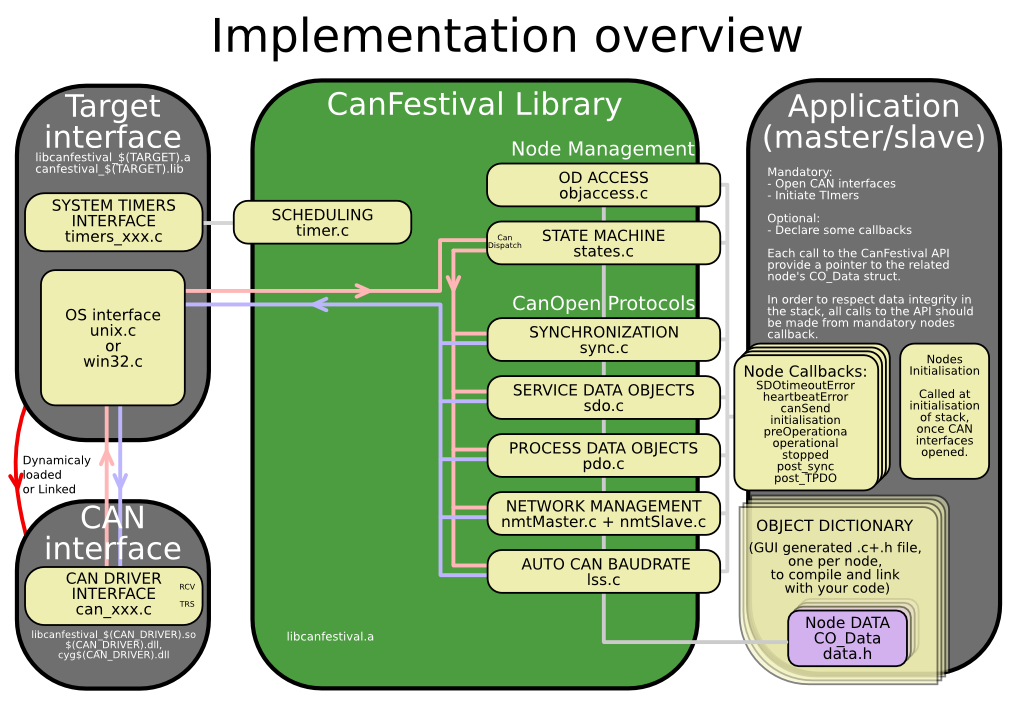
\includegraphics[width=12cm]{Pictures/10000201000003F9000002CF880931E7.png}
\end{center}

\bigskip

\subsection{CanFestival CAN interfaces}
Because most CAN controllers and drivers implement FIFOs, CanFestival
consider sending message as a non bloking operation.

In order to prevent reentrent calls to the stack, messages reception is
implemented differently on {\textmu}C and OS.:

\liststyleLvi
\begin{enumerate}
\item {\textmu}C must provide interuption masking for timer and can
receive IT\newline
 \begin{center}
   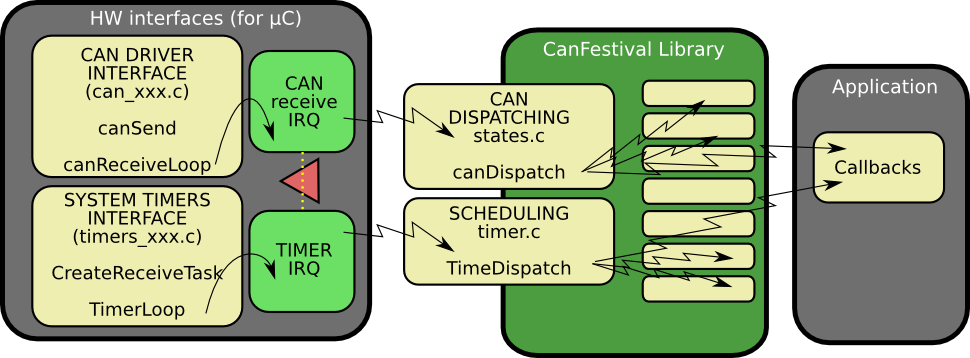
\includegraphics[width=12cm]{Pictures/10000201000003CA0000016604E6A5EF.png}
\end{center}
\item OS must provide a receive thread, a timer thread and a mutex. CAN
reception is a bloking operation.\newline
\begin{center}
   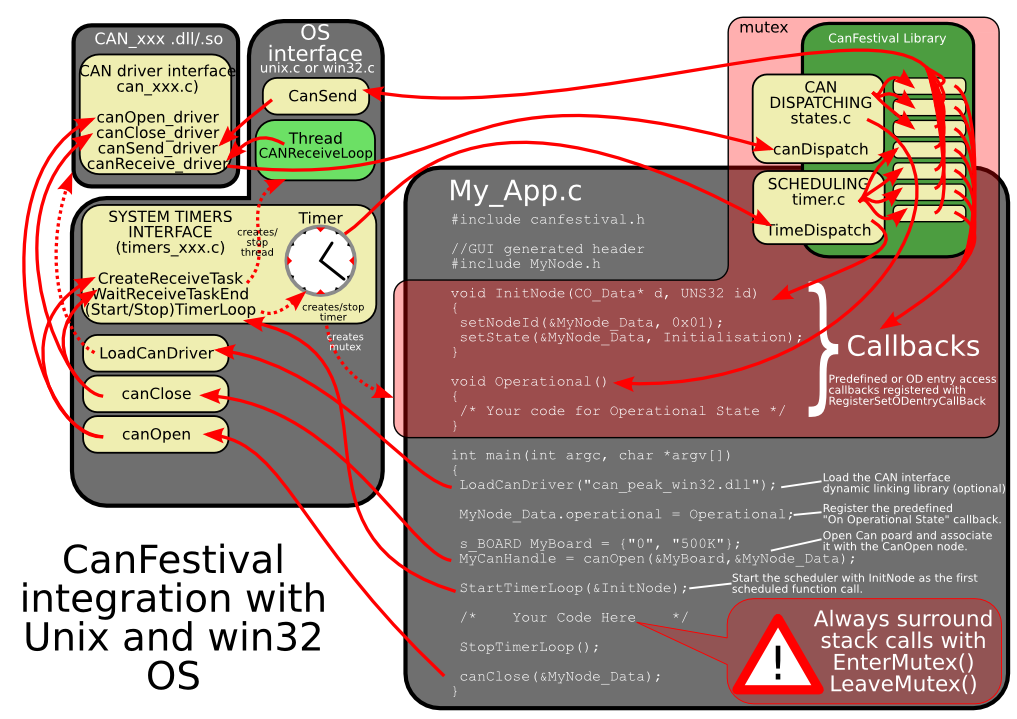
\includegraphics[width=12cm]{Pictures/10000201000003F9000002CF8B0CDAEA.png}
\end{center}
\end{enumerate}
\subsection{CanFestival events scheduling}
A CanOpen node must be able to take delayed actions.

As exemples, periodic sync emission, heartbeat production or SDO timeout
need to set some alarms that will be called later and do the job.

{\textmu}C generaly do not have enough free timers to handle all the
CanOpen needs directly. Moreover, CanFestival internal data may be
corrupt by reentrant calls. 

CanFestival implement a micro{}-scheduler (timer.c). It uses only one
timer to mimic many timers. It manage an alarm table, and call alarms
at desired time.

\begin{center}
   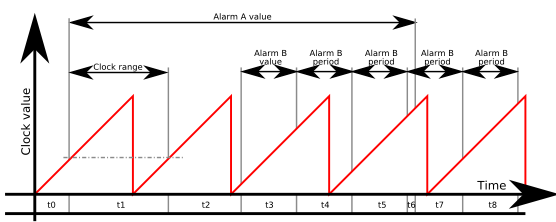
\includegraphics[width=12cm]{Pictures/100000000000022C000000DEDAD2140C.png}
\end{center}

Scheduler can handle short clock value ranges limitation found on some
{\textmu}C. As an example, value range for a 16bit clock counter with
4{\textmu}s tick is crossed within 0.26 seconds... Long alarms must be
segmented.

Chronogram illustrate a long alarm (A) and a short periodic alarm (B),
with a A value {\textgreater} clock range {\textgreater} B value.
Values t0...t8 are successive setTimer call parameter values. t1
illustrates an intermediate call to TimeDispatch, caused by a delay
longer than clock range. Because of long alarm segmentation, at the end
of t1, TimeDispatch call will not trig any alarm callback.

\begin{center}
   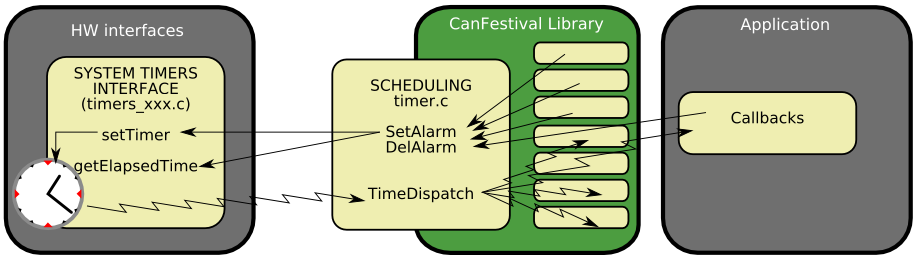
\includegraphics[width=12cm]{Pictures/1000000000000396000000FFC42573DA.png}
\end{center}

\section{Linux Target}
Linux target is default configure target.

\subsection{Linux Compilation and installation}
Call ./configure {--}help to see all available compile time options.

After invoking ./configure with your platform specific switches, just
type make.

{\ttfamily
./configure [options]}

{\ttfamily
make}

{\ttfamily
make install}

\subsubsection{Standard Linux node}
Configure switch:

{\ttfamily
 {}-{}-timers=unix}

To do a CANopen node running on PC{}-Linux, you need :

\liststyleLvii
\begin{enumerate}
\item A working linux distribution
\item One or more Peak system PC CAN interface and the last Peak Linux
driver installed.
\end{enumerate}
\subsubsection{Real{}-Time Linux node}
Configure switch:

{\ttfamily
 {}-{}-timers=xeno}

To do a CANopen node running on PC{}-Linux, you need :

\liststyleLviii
\begin{enumerate}
\item A working Linux distribution patched with XENOMAI 2.1 or greater.
\item One or more Peak system PC CAN interface and the last Peak Real
Time Linux driver installed.
\end{enumerate}
\subsubsection{CAN devices}
Curently supported CAN devices and corresponding configure switch:

\paragraph{Peak systems}
Configure switch:

{\ttfamily
{}-{}-can=peak\_linux}

PeakSystems CAN interface is automatically chosen as default CAN
interface if libpcan is present in the system.

Please download driver at
\href{http://www.peak-system.com/linux}{http://www.peak{}-system.com/linux}
and follow instructions in order to install driver on your system.

\paragraph{Socket{}-Can (http://socketcan.berlios.de)}
Configure switch:

{\ttfamily
{}-{}-can=socket}

\paragraph{LinCan}
Configure switch:

{\ttfamily
{}-{}-can=lincan}

\paragraph{Virtual CAN interfaces (for test/debug)}
Configure switch:

{\ttfamily
{}-{}-can=virtual}

Virtual CAN interface use Unix pipes to emulate a virtual CAN network.
Each message issued from a node is repeat to all other nodes. Currently
only works with nodes running in the same process, and does not support
work with Xenomai.

\subsection{Testing your CanFestival installation}
Sample provided in /example/TestMasterSlave is installed into your
system during installation.

{\ttfamily
TestMasterSlave}

Default can driver library is libcanfestival\_can\_virtual.so., which
will simply pass CAN messages through Unix pipes between Master and
Slave. 

You may also want to specify different can interface and define some CAN
ports. An other example using Peak{\textquotesingle}s dual PCMCIA
(configure and install with {--}can=peak) :

{\ttfamily
TestMasterSlave {}-l libcanfestival\_can\_peak.so {}-s 40 {}-m 41}

\section{Windows Targets}
CanFestival can be compiled and run on Windows platform. It is possible
to use both Cygwin and win32 native runtime environment.

\subsection{Object Dictionary Editor GUI installation.}
Please refer to
\hyperlink{a821UsingDictionaryEditorGUIoutline}{8.2.1)Using Dictionary
Editor GUI}

\subsection{CYGWIN}
\subsubsection{Requirements}
Cygwin have to be installed with those packages :

\liststyleLix
\begin{enumerate}
\item gcc
\item unzip
\item wget
\item make
\end{enumerate}
Currently, the only supported CAN devices are PeakSystems ones, with
PcanLight driver and library. 

Please download driver at
\href{http://www.peak-system.com/themen/download_gb.html}{http://www.peak{}-system.com/themen/download\_gb.html}
\space and follow instructions in order to install driver on your system.

Install Cygwin as required, and the driver for your Peak CAN device.

Open a Cygwin terminal, and follow those instructions:

\subsubsection{Cygwin configuration and compilation}
\paragraph{A single node with PcanLight and Peak CAN{}-USB adapter}
Download the PCAN{}-Light Zip file for your HW ( URL from download page
): 

{\ttfamily
wget http://www.peak{}-system.com/files/usb.zip}

Extract its content into your cygwin home (it will create a ``Disk''
directory):

{\ttfamily
unzip usb.zip}

Configure CanFestival3 providing path to the desired PcanLight
implementation:

{\ttfamily
cd CanFestival{}-3}

{\ttfamily
export PCAN\_INCLUDE=\~{}/Disk/PCAN{}-Light/Api/}

{\ttfamily
export PCAN\_HEADER=Pcan\_usb.h}

{\ttfamily
export PCAN\_LIB=\~{}/Disk/PCAN{}-Light/Lib/Visual{\textbackslash}
C++/Pcan\_usb.lib}

{\ttfamily
./configure {}-{--}can=peak\_win32}

{\ttfamily
make}

In order to test, you have to use another CanFestival node, connect with
a CAN cable.

{\ttfamily
cp \~{}/Disk/PCAN{}-Light/Pcan\_usb.dll .}

{\ttfamily
./examples/TestMasterSlave/TestMasterSlave {\textbackslash}}

{\ttfamily
  {}-l drivers/can\_peak\_win32/cygcan\_peak\_win32.dll
{\textbackslash}}

{\ttfamily
  {}-S 500K {}-M none}

Then, on the other node :

{\ttfamily
./TestMasterSlave {}-l my\_driver.so {}-S none {}-M 500K}

Now messages are beeing exchanged between master and slave node.

\paragraph{Two nodes with PcanLight and Peak dual PCMCIA{}-CAN adapter}
Download the PCAN{}-Light Zip file for your HW ( URL from download page
): 

{\ttfamily
wget http://www.peak{}-system.com/files/pccard.zip}

Extract its content into your cygwin home (it will create a ``Disk''
directory):

{\ttfamily
unzip pccard.zip}

The configure CanFestival3 providing path to the desired PcanLight
implementation:

{\ttfamily
export PCAN\_INCLUDE=\~{}/Disk/PCAN{}-Light/Api/\newline
export PCAN\_HEADER=Pcan\_pcc.h\newline
export PCAN\_LIB=\~{}/Disk/PCAN{}-Light/Lib/Visual{\textbackslash}
C++/Pcan\_pcc.lib\newline
export PCAN2\_HEADER=Pcan\_2pcc.\newline
export PCAN2\_LIB=\~{}/Disk/PCAN{}-Light/Lib/Visual{\textbackslash}
C++/Pcan\_2pcc.lib}

In order to test, just connect together both CAN ports of the PCMCIA
card. Don{\textquotesingle}t forget 120ohms terminator.

{\ttfamily
cp \~{}/Disk/PCAN{}-Light/Pcan\_pcc.dll .}

{\ttfamily
cp \~{}/Disk/PCAN{}-Light/Pcan\_2pcc.dll .}

{\ttfamily
./examples/TestMasterSlave/TestMasterSlave {\textbackslash}}

{\ttfamily
  {}-l drivers/can\_peak\_win32/cygcan\_peak\_win32.dll}

Messages are then exchanged between master and slave node, both inside
TestMasterSlave{\textquotesingle}s process.

\subsection{Visual Studio C++}
\subsubsection{Requirements}
Minimal Cygwin installation is required at configuration time in order
to create specific header files (config.h and cancfg.h). Once this
files created, cygwin is not necessary any more.

Project and solution files have been created and tested with Visual
Studio Express 2005. Be sure to have installed Microsoft Platform SDK,
as recommended at the end of Visual Studio installation.

\subsubsection{Configuration with cygwin}
Follow instructions given at 
\hyperlink{Cygwin configuration and compilation}{Cygwin
configuration and compilation}, but do neither call make nor do tests,
just do configuration steps. This will create headers files accordingly
to your configuration parameters, and the desired CAN hardware.

\subsubsection{Compilation with Visual Studio}
You can either load independents ``*.vcproj'' project files along your
own projects in your own solution or load the provided
``CanFestival{}-3.vc8.sln'' solution files directly.

Build CanFestival{}-3 project first.

\paragraph{PcanLight and the can\_peak\_win32 project.}
Chosen Pcan\_xxx.lib and eventually Pcan\_2xxx.lib files must be added
to can\_peak\_win32 \space \space project before build of the DLL.

\subsubsection{Testing}
Copy eventually needed dlls (ie : Pcan\_Nxxx.lib) into Release or Debug
directory, and run the test program:

{\ttfamily
TestMasterSlave.exe {}-l can\_peak\_win32.dll}

\section{Motorola HCS12}
The examples have been tested on a MC9S12DG255 mounted on a
Elektronikladen HCS12 T{}-board.

Beware that there are a few differences in the MSCAN module of the
68HC12 and HCS12 microcontroller. For a HC12, you must adapt the driver
that we provide for \space the HCS12.

For the difference MSCAN HC12/HCS12, see the Motorola application note
AN2011/D.

Configure switch:

{\ttfamily
 {}-{}-target=hcs12}

To do a CANopen node running on a microncontroller Motorola MC9S12DP256,
you need :

\liststyleLx
\begin{enumerate}
\item The compiler GNU gcc for HC11, HC12, HCS12 : m6811{}-elf. \newline
Download the \textbf{release 3.1} at :
\space \href{http://m68hc11.serveftp.org/m68hc11_pkg_rpm.php}{http://m68hc11.serveftp.org/m68hc11\_pkg\_rpm.php}

\item A board with this chip. We are using the T{}-board from
Electronikladden. 
\item At least about 40 kBytes of program memory.
\item A tool to flash the memory. (We are using the hight cost
Lauterbach debugger).
\end{enumerate}
\subsection{Running a HCS12 node}
\subsubsection{Compiling Canfestival:}
{\ttfamily
./configure {--}target=hcs12}

\subsubsection{Compiling and building an example}
Enter in the folder of an HCS12 example, 

{\ttfamily
make all}

\subsubsection{Flashing the memory :}
Use your prefered loader ! If you are using a debugger Lauterbach, you
can load the bash file : trace32\_flash\_programmer.cmm. It loads
directly the elf file.

\subsubsection{Connecting to a serial RS232 console :}
Connect the portS(TxD0) of the HCS12 to a console configured at 19200
bauds 8N1, via a Max232 chip to adapt the electricals levels. On Linux,
you can use minicom. Connecting to a console is usefull to read the
messages, but not required.

\subsubsection{Connecting to the CAN network :}
Connect the port CAN0 (pin PM0, PM1) to the network via a CAN
controller. On our board, the CAN controler is a PCA82C250 chip.

\subsubsection{starting the node :}
Press the reset of your HCS12 board.

\section{Example and test program:}
The ``examples'' directory contains some test program you can use as
example for your own developments.

\subsection{TestMasterSlave}
{\ttfamily
**************************************************************\space}

{\ttfamily
* \space TestMasterSlave
\space \space \space \space \space \space \space \space \space \space \space \space \space \space \space \space \space \space \space \space \space \space \space \space \space \space \space \space \space \space \space \space \space \space \space \space \space \space \space \space \space \space *}

{\ttfamily
*
\space \space \space \space \space \space \space \space \space \space \space \space \space \space \space \space \space \space \space \space \space \space \space \space \space \space \space \space \space \space \space \space \space \space \space \space \space \space \space \space \space \space \space \space \space \space \space \space \space \space \space \space \space \space \space \space \space \space \space *}

{\ttfamily
* \space A simple example for PC. It does implement 2 CanOpen \space \space \space \space \space *}

{\ttfamily
* \space nodes in the same process. A master and a slave. Both \space \space \space \space *}

{\ttfamily
* \space communicate together, exchanging periodically NMT, SYNC, \space *}

{\ttfamily
* \space SDO and PDO. Master configure heartbeat producer time \space \space \space \space *}

{\ttfamily
* \space at 1000 ms for slave node{}-id 0x02 by concise DCF.
\space \space \space \space \space \space \space \space *}

{\ttfamily
*
\space \space \space \space \space \space \space \space \space \space \space \space \space \space \space \space \space \space \space \space \space \space \space \space \space \space \space \space \space \space \space \space \space \space \space \space \space \space \space \space \space \space \space \space \space \space \space \space \space \space \space \space \space \space \space \space \space \space \space *}

{\ttfamily
* \space \space Usage:
\space \space \space \space \space \space \space \space \space \space \space \space \space \space \space \space \space \space \space \space \space \space \space \space \space \space \space \space \space \space \space \space \space \space \space \space \space \space \space \space \space \space \space \space \space \space \space \space \space \space *}

{\ttfamily
* \space \space ./TestMasterSlave \space [OPTIONS]
\space \space \space \space \space \space \space \space \space \space \space \space \space \space \space \space \space \space \space \space \space \space \space \space \space \space \space \space *}

{\ttfamily
*
\space \space \space \space \space \space \space \space \space \space \space \space \space \space \space \space \space \space \space \space \space \space \space \space \space \space \space \space \space \space \space \space \space \space \space \space \space \space \space \space \space \space \space \space \space \space \space \space \space \space \space \space \space \space \space \space \space \space \space *}

{\ttfamily
* \space \space OPTIONS:
\space \space \space \space \space \space \space \space \space \space \space \space \space \space \space \space \space \space \space \space \space \space \space \space \space \space \space \space \space \space \space \space \space \space \space \space \space \space \space \space \space \space \space \space \space \space \space \space *}

{\ttfamily
* \space \space \space \space {}-l : Can library
[{\textquotedbl}libcanfestival\_can\_virtual.so{\textquotedbl}]
\space \space \space \space *}

{\ttfamily
*
\space \space \space \space \space \space \space \space \space \space \space \space \space \space \space \space \space \space \space \space \space \space \space \space \space \space \space \space \space \space \space \space \space \space \space \space \space \space \space \space \space \space \space \space \space \space \space \space \space \space \space \space \space \space \space \space \space \space \space *}

{\ttfamily
* \space \space \space Slave:
\space \space \space \space \space \space \space \space \space \space \space \space \space \space \space \space \space \space \space \space \space \space \space \space \space \space \space \space \space \space \space \space \space \space \space \space \space \space \space \space \space \space \space \space \space \space \space \space \space *}

{\ttfamily
* \space \space \space \space {}-s : bus name [{\textquotedbl}0{\textquotedbl}]
\space \space \space \space \space \space \space \space \space \space \space \space \space \space \space \space \space \space \space \space \space \space \space \space \space \space \space \space \space \space \space \space \space \space \space *}

{\ttfamily
* \space \space \space \space {}-S : 1M,500K,250K,125K,100K,50K,20K,10K,none(disable) \space *}

{\ttfamily
*
\space \space \space \space \space \space \space \space \space \space \space \space \space \space \space \space \space \space \space \space \space \space \space \space \space \space \space \space \space \space \space \space \space \space \space \space \space \space \space \space \space \space \space \space \space \space \space \space \space \space \space \space \space \space \space \space \space \space \space *}

{\ttfamily
* \space \space \space Master:
\space \space \space \space \space \space \space \space \space \space \space \space \space \space \space \space \space \space \space \space \space \space \space \space \space \space \space \space \space \space \space \space \space \space \space \space \space \space \space \space \space \space \space \space \space \space \space \space *}

{\ttfamily
* \space \space \space \space {}-m : bus name [{\textquotedbl}1{\textquotedbl}]
\space \space \space \space \space \space \space \space \space \space \space \space \space \space \space \space \space \space \space \space \space \space \space \space \space \space \space \space \space \space \space \space \space \space \space *}

{\ttfamily
* \space \space \space \space {}-M : 1M,500K,250K,125K,100K,50K,20K,10K,none(disable) \space *}

{\ttfamily
*
\space \space \space \space \space \space \space \space \space \space \space \space \space \space \space \space \space \space \space \space \space \space \space \space \space \space \space \space \space \space \space \space \space \space \space \space \space \space \space \space \space \space \space \space \space \space \space \space \space \space \space \space \space \space \space \space \space \space \space *}

{\ttfamily
**************************************************************}


\bigskip

{\sffamily
Notes for Concise DCF :}


\bigskip

{\sffamily
 In this example, Master configure \space heartbeat producer time at 1000 ms
for slave node{}-id 0x02 by concise DCF according DS{}-302 profile. }

{\sffamily
 }

{\sffamily
 Index 0x1F22 , sub{}-index 0x00 of the master OD, correspond to the
number of entries. This equal to the maximum possible nodeId (127).
Each sub{}-index points to the Node{}-ID of the device, to which the
configuration belongs. }


\bigskip

{\sffamily
 To add more parameters configurations to the slave, the value at
sub{}-index 0x02 must be a binary stream (little{}-endian) following
this structure :\newline
\{
(UNS32) nb of entries\newline
(UNS16) index parameter 1\newline
(UNS8) sub{}-index parameter 1\newline
(UNS32) size data parameter 1\newline
(DOMAIN) data parameter 1\newline
(UNS16) index parameter 2\newline
(UNS8) sub{}-index parameter 2\newline
(UNS32) size data parameter 2\newline
(DOMAIN) data parameter 2\newline
\space \space \space \space \space ....\newline
(UNS16) index parameter n\newline
(UNS8) sub{}-index parameter n\newline
(UNS32) size data parameter n\newline
(DOMAIN) data parameter n\newline
\}
}

{\sffamily
 So the binary value stream to configure heartbeat producer time must be
:\newline
    0100000017100002000000e803}

{\sffamily
The slave node is configured just before the Master entering in
Pre\_operational state.}

\subsection{gene\_SYNC\_HCS12 :}
This is a simple CanOpen node that only send cyclic SYNC message. It
demonstrate implementation on HCS12 based board.


\bigskip

\subsection{TestMasterMicroMod }
{\ttfamily
**************************************************************}

{\ttfamily
* \space TestMasterMicroMod
\space \space \space \space \space \space \space \space \space \space \space \space \space \space \space \space \space \space \space \space \space \space \space \space \space \space \space \space \space \space \space \space \space \space \space \space \space \space \space *}

{\ttfamily
*
\space \space \space \space \space \space \space \space \space \space \space \space \space \space \space \space \space \space \space \space \space \space \space \space \space \space \space \space \space \space \space \space \space \space \space \space \space \space \space \space \space \space \space \space \space \space \space \space \space \space \space \space \space \space \space \space \space \space \space *}

{\ttfamily
* \space A simple example for PC.
\space \space \space \space \space \space \space \space \space \space \space \space \space \space \space \space \space \space \space \space \space \space \space \space \space \space \space \space \space \space \space \space \space *}

{\ttfamily
* \space A CanOpen master that control a MicroMod module:
\space \space \space \space \space \space \space \space \space *}

{\ttfamily
* \space {}- setup module TPDO 1 transmit type
\space \space \space \space \space \space \space \space \space \space \space \space \space \space \space \space \space \space \space \space \space \space *}

{\ttfamily
* \space {}- setup module RPDO 1 transmit type
\space \space \space \space \space \space \space \space \space \space \space \space \space \space \space \space \space \space \space \space \space \space *}

{\ttfamily
* \space {}- setup module hearbeatbeat period
\space \space \space \space \space \space \space \space \space \space \space \space \space \space \space \space \space \space \space \space \space \space \space *}

{\ttfamily
* \space {}- disable others TPDOs
\space \space \space \space \space \space \space \space \space \space \space \space \space \space \space \space \space \space \space \space \space \space \space \space \space \space \space \space \space \space \space \space \space \space \space *}

{\ttfamily
* \space {}- set state to operational
\space \space \space \space \space \space \space \space \space \space \space \space \space \space \space \space \space \space \space \space \space \space \space \space \space \space \space \space \space \space \space *}

{\ttfamily
* \space {}- send periodic SYNC
\space \space \space \space \space \space \space \space \space \space \space \space \space \space \space \space \space \space \space \space \space \space \space \space \space \space \space \space \space \space \space \space \space \space \space \space \space *}

{\ttfamily
* \space {}- send periodic RPDO 1 to Micromod (digital output) \space \space \space \space \space \space *}

{\ttfamily
* \space {}- listen Micromod{\textquotesingle}s TPDO 1 (digital input)
\space \space \space \space \space \space \space \space \space \space \space \space \space \space \space *}

{\ttfamily
* \space {}- Mapping RPDO 1 bit per bit (digital input)
\space \space \space \space \space \space \space \space \space \space \space \space \space *}

{\ttfamily
*
\space \space \space \space \space \space \space \space \space \space \space \space \space \space \space \space \space \space \space \space \space \space \space \space \space \space \space \space \space \space \space \space \space \space \space \space \space \space \space \space \space \space \space \space \space \space \space \space \space \space \space \space \space \space \space \space \space \space \space *}

{\ttfamily
* \space \space Usage:
\space \space \space \space \space \space \space \space \space \space \space \space \space \space \space \space \space \space \space \space \space \space \space \space \space \space \space \space \space \space \space \space \space \space \space \space \space \space \space \space \space \space \space \space \space \space \space \space \space \space *}

{\ttfamily
* \space \space ./TestMasterMicroMod \space [OPTIONS]
\space \space \space \space \space \space \space \space \space \space \space \space \space \space \space \space \space \space \space \space \space \space \space \space \space *}

{\ttfamily
*
\space \space \space \space \space \space \space \space \space \space \space \space \space \space \space \space \space \space \space \space \space \space \space \space \space \space \space \space \space \space \space \space \space \space \space \space \space \space \space \space \space \space \space \space \space \space \space \space \space \space \space \space \space \space \space \space \space \space \space *}

{\ttfamily
* \space \space OPTIONS:
\space \space \space \space \space \space \space \space \space \space \space \space \space \space \space \space \space \space \space \space \space \space \space \space \space \space \space \space \space \space \space \space \space \space \space \space \space \space \space \space \space \space \space \space \space \space \space \space *}

{\ttfamily
* \space \space \space \space {}-l : Can library
[{\textquotedbl}libcanfestival\_can\_virtual.so{\textquotedbl}]
\space \space \space \space *}

{\ttfamily
*
\space \space \space \space \space \space \space \space \space \space \space \space \space \space \space \space \space \space \space \space \space \space \space \space \space \space \space \space \space \space \space \space \space \space \space \space \space \space \space \space \space \space \space \space \space \space \space \space \space \space \space \space \space \space \space \space \space \space \space *}

{\ttfamily
* \space \space \space Slave:
\space \space \space \space \space \space \space \space \space \space \space \space \space \space \space \space \space \space \space \space \space \space \space \space \space \space \space \space \space \space \space \space \space \space \space \space \space \space \space \space \space \space \space \space \space \space \space \space \space *}

{\ttfamily
* \space \space \space \space {}-i : Slave Node id format [0x01 , 0x7F]
\space \space \space \space \space \space \space \space \space \space \space \space \space \space \space *}

{\ttfamily
*
\space \space \space \space \space \space \space \space \space \space \space \space \space \space \space \space \space \space \space \space \space \space \space \space \space \space \space \space \space \space \space \space \space \space \space \space \space \space \space \space \space \space \space \space \space \space \space \space \space \space \space \space \space \space \space \space \space \space \space *}

{\ttfamily
* \space \space \space Master:
\space \space \space \space \space \space \space \space \space \space \space \space \space \space \space \space \space \space \space \space \space \space \space \space \space \space \space \space \space \space \space \space \space \space \space \space \space \space \space \space \space \space \space \space \space \space \space \space *}

{\ttfamily
* \space \space \space \space {}-m : bus name [{\textquotedbl}1{\textquotedbl}]
\space \space \space \space \space \space \space \space \space \space \space \space \space \space \space \space \space \space \space \space \space \space \space \space \space \space \space \space \space \space \space \space \space \space \space *}

{\ttfamily
* \space \space \space \space {}-M : 1M,500K,250K,125K,100K,50K,20K,10K
\space \space \space \space \space \space \space \space \space \space \space \space \space \space \space *}

{\ttfamily
*
\space \space \space \space \space \space \space \space \space \space \space \space \space \space \space \space \space \space \space \space \space \space \space \space \space \space \space \space \space \space \space \space \space \space \space \space \space \space \space \space \space \space \space \space \space \space \space \space \space \space \space \space \space \space \space \space \space \space \space *}

{\ttfamily
**************************************************************}

\section{Developing a new node}
Using provided examples as a base for your new node is generally a good
idea. You can also use the provided *.od files as a base for your node
object dictionary.

Creating a new CanOpen node implies to define the Object Dictionary of
this node. For that, developer have to provide a C file. This C file
contains the definition of all dictionary entries, and some kind of
index table that helps the stack to access some entries directly.

\subsection{Using Dictionary Editor GUI}
The Object Dictionary Editor is a WxPython based GUI that is used to
create the C file needed to create a new CanOpen node. 

\subsubsection{Installation and usage on Linux}
You first have to download and install Gnosis XML modules. This is
automated by a Makefile rule.

{\ttfamily
cd objdictgen}

{\ttfamily
make}

Now start the editor.

{\ttfamily
python objdictedit.py [od files...]}

\subsubsection{Installation and usage on Windows}
Install Python (at least version 2.4) and wxPython (at least version
2.6.3.2).

Cygwin users can install Gnosis XML utils the same as Linux use. Just
call make.

{\ttfamily
cd objdictgen}

{\ttfamily
make}

Others will have to download and intall Gnosis XML by hand :

{\ttfamily
Gnosis Utils:}

{\ttfamily
http://freshmeat.net/projects/gnosisxml/}

{\ttfamily
http://www.gnosis.cx/download/Gnosis\_Utils.More/Gnosis\_Utils{}-1.2.1.win32{}-py24.exe}

{\ttfamily
Get latest version.}

Download CanFestival archive and uncompress it. Use windows file
explorer to go into CanFestival3{\textbackslash}objdicgten, and
double{}-click on objdictedit.py.

\subsubsection{About}
The Object Dictionary editor GUI is a python application that use the
Model{}-View{}-Controller design pattern. It depends on WxPython to
display view on any supported platform.

 \begin{center}
   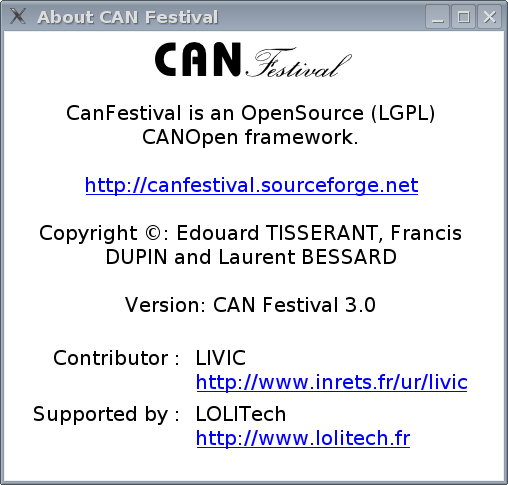
\includegraphics[width=7cm]{Pictures/10000201000001FC000001E5D65E8766.png}
\end{center}

\subsubsection{Main view}
Top list let you choose dictionary section, bottom left list is the
selected index in that dictionary, and bottom right list are edited
sub{}-indexes.

 \begin{center}
   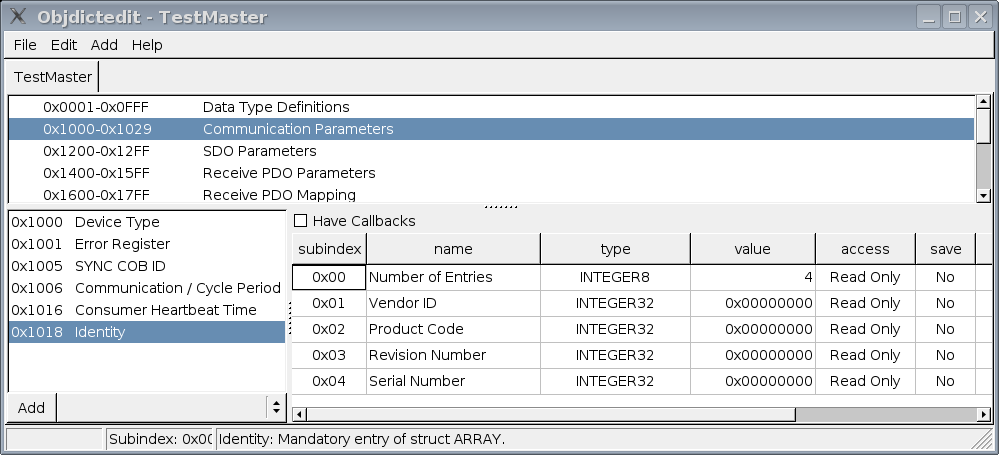
\includegraphics[width=12cm]{Pictures/10000201000003E7000001C7B0296577.png}
\end{center}

 \begin{center}
   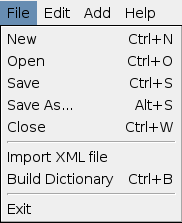
\includegraphics[width=3cm]{Pictures/10000000000000B6000000DF1EDD1E73.png}
\end{center}
  \begin{center}
   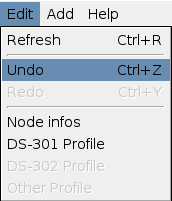
\includegraphics[width=3cm]{Pictures/10000000000000AC000000C9C3F53FA6.png}
\end{center}
 \begin{center}
   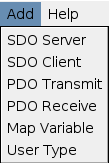
\includegraphics[width=3cm]{Pictures/100000000000006D000000A31EC8CB54.png}
\end{center}
  \begin{center}
   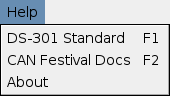
\includegraphics[width=3cm]{Pictures/10000000000000AA0000006014F74635.png}
\end{center}

\subsubsection{New node}
Edit your node name, ID and type. Choose your inherited specific
profile.

 \begin{center}
   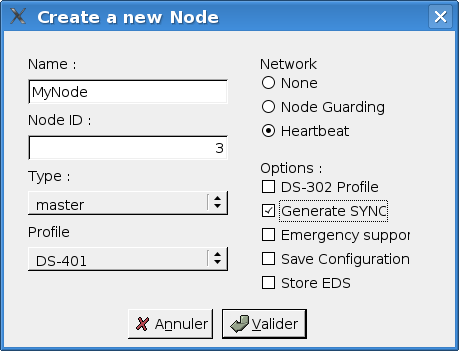
\includegraphics[width=11cm]{Pictures/10000201000001CB0000015F4FC09B68.png}
\end{center}

\subsubsection{Node info}
Edit your node name, ID and type.

 \begin{center}
   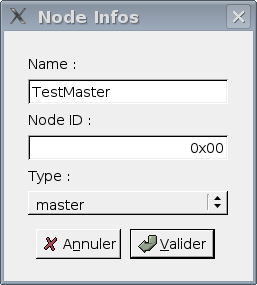
\includegraphics[width=7cm]{Pictures/10000201000001010000011DA724D25C.png}
\end{center}

\subsubsection{Profile editor}
Chose the used profile to edit.\newline
 \begin{center}
   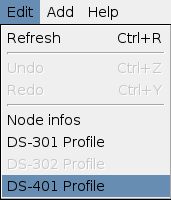
\includegraphics[width=4cm]{Pictures/10000000000000AB000000C88F594413.png}
\end{center}

Pick up optional chosen profile entries.\newline
 \begin{center}
   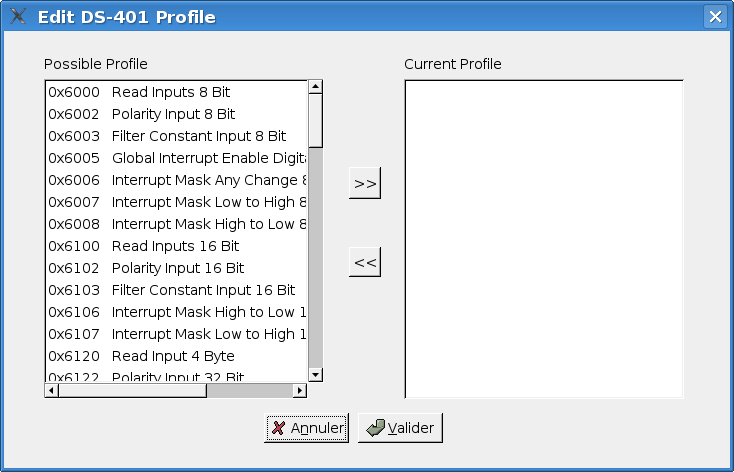
\includegraphics[width=11cm]{Pictures/10000201000002DE000001D82D89C224.png}
\end{center}

\subsubsection{User types}
Use User Types to implement value boundaries, and string lentgth\newline
 \begin{center}
   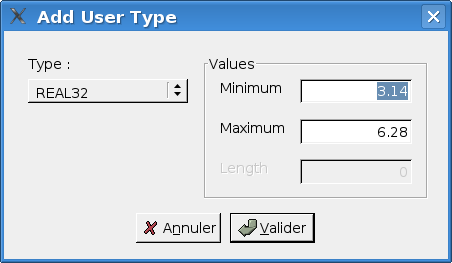
\includegraphics[width=11cm]{Pictures/10000201000001C40000010766961D7F.png}
\end{center}

\subsubsection{Mapped variable}
Add your own specific dictionary entries and associated mapped
variables.\newline
 \begin{center}
   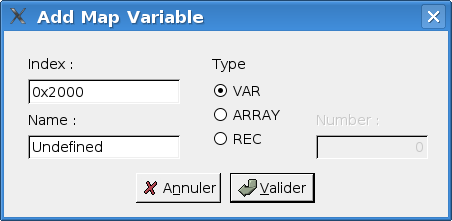
\includegraphics[width=11cm]{Pictures/10000201000001C4000000DD129D4661.png}
\end{center}

\subsubsection{Integrated help}
Using F1 key, you can get context sensitive help.\newline
 \begin{center}
   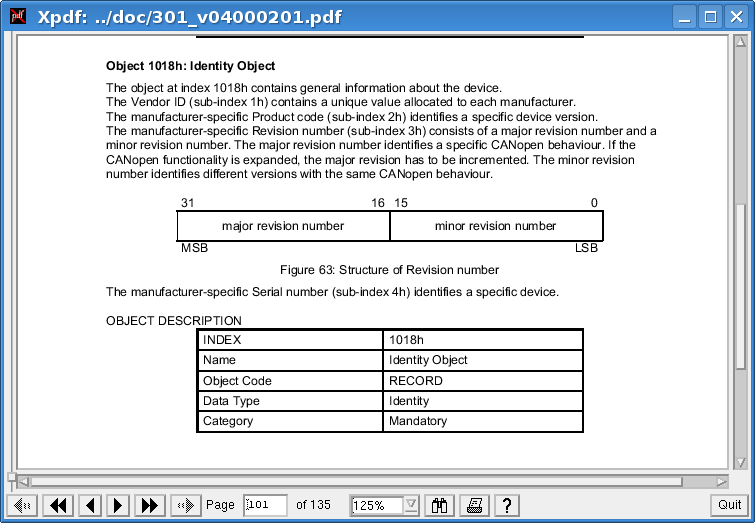
\includegraphics[width=12cm]{Pictures/10000201000002F30000020B23ED7F67.png}
\end{center}

In order to do that, official 301\_v04000201.pdf file must be placed
into doc/ directory, and xpdf must be present on your system.

F2 key open HTML CanFestival help.\newline
 \begin{center}
   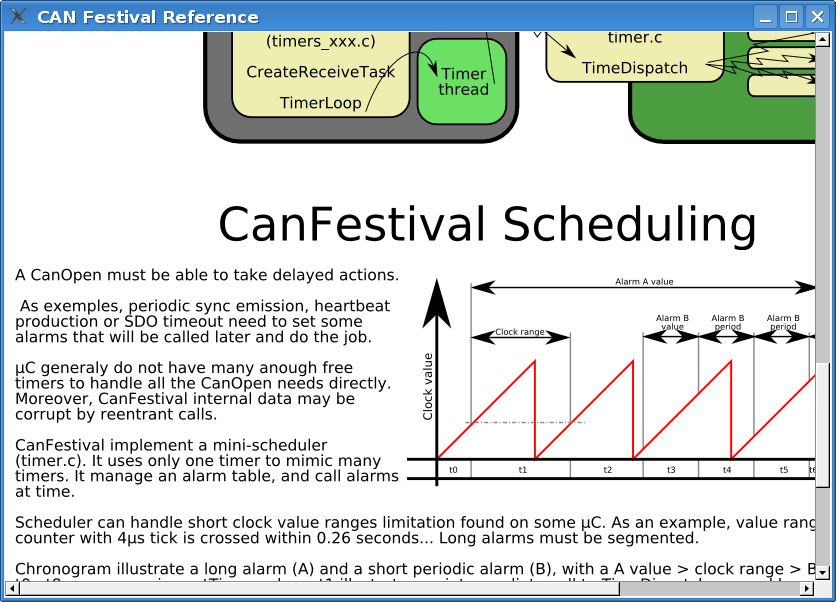
\includegraphics[width=12cm]{Pictures/10000201000003440000025ACC3FD2F1.png}
\end{center}

\subsection{Generating the object Dictionary}
Once object dictionary has been edited and saved, you have to generate
object dictionary C code for your CanFestival node.

\subsubsection{With GUI}
Menu entry ``File/Build Dictionary''.

 \begin{center}
   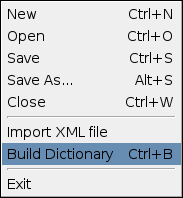
\includegraphics[width=4cm]{Pictures/10000201000000B7000000C66AF89CD5.png}
\end{center}

Choose C file to create or overwrite. Header file will be also created
with the same prefix as C file.

\subsubsection{With command line}
{\ttfamily
Usage of objdictgen.py :\newline
python objdictgen.py XMLFilePath CfilePath}

\section{FAQ}
\subsection{General}
\subsubsection{Does the code compiles on Windows ?}
Yes, with both Cygwin and Visual Studio C++.

Because CANopen layer is coded with C, put a compilation option /TC or
/TP if you plan to mix C++ files. See the MSDN documentation about
that.

\subsubsection{How to fit the library to an other microcontr\^oler ?}
First, be sure that you have at least 40K bytes of program memory, and
about 2k of RAM. 

You have to create target specific interface to HW resources. Take model
on bundled interfaces provided in drivers/ and create your own
interface. You also have to update Makefile.in files for target
specific cflags and options. Chose {--}targer= configure switch to
compile your specific interface.

You are welcome to contribute{}-back your own interfaces ! Other
Canfestival users will use it and provide feedback, tests and
enhancements.

\subsubsection{Is CanFestival3 conform to DS301 v.4.02 ?}
Thanks to Philippe Foureys (IUT of Valence), a slave node have been
tested with the National Instrument CanOpen Conformance Test. It passed
the test with success.

Some very small unconformity have been found in very unusual situations,
for example in the SDO code response to wrong messages.

\subsection{LINUX}
\subsubsection{How to use a Peaksystem CAN board ?}
Just install peak driver and then compile and install Canfestival. Peak
driver is detected at compile time.

\subsubsection{How to use an unsupported CAN board ?}
You have to install the specific driver on your system, with necessary
libs and headers. 

Use can\_peak.c/h or can\_virtual.c/h as an example, and adapt it to
your driver API.

Execute configure script and choose {}-{}-can=mydriver

\subsection{Win32}
Compatibility:

\liststyleLxi
\begin{enumerate}
\item Code was compiled MS VisualStudio 2003.NET and VisualStudio
2005.NET for WindowsXP \space with ANSI and UNICODE configurations and for
WindowsCE 5.0. 
\item Some preliminary testing was done, but not enough to be used in
mission critical projects.
\end{enumerate}
Additional Features:

\liststyleLxii
\begin{enumerate}
\item Non{}-integral integers support implementation UNS24, UNS40, UNS48
etc.
\item When enable debug output with DEBUG\_WAR\_CONSOLE\_ON or
DEBUG\_ERR\_CONSOLE\_ON, you can navigate in CanFestival source code by
double clicking at diagnostic lines in VisualStudio.NET 200X Debug
Output Window.
\end{enumerate}
Custom size integral types such as INTEGER24, UNS40, INTEGER56 etc. have
been defined as 64 bits integers. You will need to replace sizeof(TYPE)
operators to sizeof\_TYPE definitions in generated code, i.e. replace
sizeof(UNS40) with sizeof\_UNS40.


\bigskip

\subsection{HCS12}
\subsubsection{Which board are you using ?}
A T{}-board from elektronikladen with a MC9S12DP256 or MC9S12DG256.

\subsubsection{Does the code compile with an other compiler than GNU gcc
?}
It is known to work with Metrowerks CodeWarrior. Here are some tips from
Philippe Foureys. :

\paragraph{Interrupt functions}
\subparagraph{Code for GCC:}
{\ttfamily
 // prototype\newline
 void \_\_attribute\_\_((interrupt))timer3Hdl(void):\newline
 // function\newline
 void \_\_attribute\_\_((interrupt))timer3Hdl(void)\{...\}}

\subparagraph{Code for CodeWarrior}
{\ttfamily
 // protoype\newline
 void interrupt timer3Hdl(void);\newline
 // function\newline
 pragma CODE\_SEG\_\_NEAR\_SEG\_NON\_BANKED\newline
 void interrupt timer3Hdl(void)\newline
 \{...\}\newline
 pragma CODE\_SEG\_DEFAULT}

\paragraph{Interrupt lock, unlock}
\subparagraph{Code for GCC}
{\ttfamily
 void unlock (void)\newline
 \{\newline
  \space \_\_asm\_\_
\_\_volatile\_\_({\textquotedbl}cli{\textquotedbl});\newline
 \}\newline
 void lock (void)\newline
 \{\newline
  \space unsigned short mask;\newline
  \space \_\_asm\_\_
\_\_volatile\_\_({\textquotedbl}tpa{\textbackslash}n{\textbackslash}tsei{\textquotedbl}:{\textquotedbl}=d{\textquotedbl}(mask));\newline
 \}}

\subparagraph{Code for CodeWarrior}
{\ttfamily
void unlock (void)\newline
 \{\newline
  \space \_\_asm({\textquotedbl}cli{\textquotedbl});\newline
 \}\newline
 void lock (void)\newline
 \{\newline
  \space unsigned short mask;\newline
  \space \_\_asm\newline
  \{\newline
  \space tpa:tsei:{\textquotedbl}=d{\textquotedbl}(mask);\newline
  \}\newline
 \}}

\paragraph{Initialize function}
\subparagraph{Code for GCC}
{\ttfamily
void initCanHCS12 (void)\newline
 \{ \space \newline
  \space //Init the HCS12 microcontroler for CanOpen \newline
  \space initHCS12();\newline
  \space \space // Init the HCS12 \space CAN driver\newline
  \space const canBusInit bi0 = \{\newline
  \space \space \space 0, \space \space \space /* no low power \space \space \space \space \space \space \space \space \space \space \space \space \space \space \space \space */
\newline
  \space \space \space 0, \space \space \space /* no time stamp
\space \space \space \space \space \space \space \space \space \space \space \space \space \space \space */\newline
  \space \space \space 1, \space \space \space /* enable MSCAN
\space \space \space \space \space \space \space \space \space \space \space \space \space \space \space \space */\newline
  \space \space \space 0, \space \space \space /* clock source : oscillator (In fact, it is not used)
\space \space */\newline
  \space \space \space 0, \space \space \space /* no loop back
\space \space \space \space \space \space \space \space \space \space \space \space \space \space \space \space */\newline
  \space \space \space 0, \space \space \space /* no listen only
\space \space \space \space \space \space \space \space \space \space \space \space \space \space */\newline
  \space \space \space 0, \space \space \space /* no low pass filter for wk up */\newline
  \space CAN\_Baudrates[CAN\_BAUDRATE\_250K],\newline
  \space \space \space \{\newline
  \space \space \space \space \space 0x00, \space \space \space /* Filter on 16 bits.\newline
  \space \space \space \space \space \space \space \space \space \space \space \space \space \space \space \space \space See Motorola Block Guide V02.14 fig
4{}-3 */\newline
  \space \space \space \space \space 0x00, 0xFF, /* filter 0 hight accept all msg
\space \space \space \space \space */\newline
  \space \space \space \space \space 0x00, 0xFF, /* filter 0 low accept all msg
\space \space \space \space \space \space \space */\newline
  \space \space \space \space \space 0x00, 0xFF, /* filter 1 hight filter all of \space msg
\space */\newline
  \space \space \space \space \space 0x00, 0xFF, /* filter 1 low filter all of \space msg
\space \space \space */\newline
  \space \space \space \space \space 0x00, 0xFF, /* filter 2 hight filter most of \space msg
*/\newline
  \space \space \space \space \space 0x00, 0xFF, /* filter 2 low filter most of \space msg
\space \space */\newline
  \space \space \space \space \space 0x00, 0xFF, /* filter 3 hight filter most of \space msg
*/\newline
  \space \space \space \space \space 0x00, 0xFF, /* filter 3 low filter most of \space msg
\space \space */\newline
  \space \space \space \}\newline
  \space \};}

\subparagraph{Code for CodeWarrior}
{\ttfamily
void initCanHCS12 (void)\newline
 \{ \space \newline
  \space //Init the HCS12 microcontroler for CanOpen \newline
  \space initHCS12();\newline
  \space \space // Init the HCS12 \space CAN driver\newline
  \space const canBusInit bi0 = \{\newline
  \space \space \space 0, \space \space \space /* no low power \space \space \space \space \space \space \space \space \space \space \space \space \space \space \space \space */
\newline
  \space \space \space 0, \space \space \space /* no time stamp
\space \space \space \space \space \space \space \space \space \space \space \space \space \space \space */\newline
  \space \space \space 1, \space \space \space /* enable MSCAN
\space \space \space \space \space \space \space \space \space \space \space \space \space \space \space \space */\newline
  \space \space \space 0, \space \space \space /* clock source : oscillator (In fact, it is not used)
\space \space */\newline
  \space \space \space 0, \space \space \space /* no loop back
\space \space \space \space \space \space \space \space \space \space \space \space \space \space \space \space */\newline
  \space \space \space 0, \space \space \space /* no listen only
\space \space \space \space \space \space \space \space \space \space \space \space \space \space */\newline
  \space \space \space 0, \space \space \space /* no low pass filter for wk up */\newline
  \space \space \space \{\newline
  \space \space \space \space 1, /* clksrc */\newline
  \space \space \space \space 3, /* brp \space \space \space */\newline
  \space \space \space \space 0, /* sjw \space \space \space */\newline
  \space \space \space \space 0, /* samp \space \space */\newline
  \space \space \space \space 1, /* tseg2 \space */\newline
  \space \space \space \space 12,/* tseg1 \space */\newline
  \space \space \space \},\newline
  \space \space \space \{\newline
  \space \space \space \space \space 0x00, \space \space \space /* Filter on 16 bits.\newline
  \space \space \space \space \space \space \space \space \space \space \space \space \space \space \space \space See Motorola Block Guide V02.14 fig
4{}-3 */\newline
  \space \space \space \space \space 0x00, 0xFF, /* filter 0 hight accept all msg
\space \space \space \space \space */\newline
  \space \space \space \space \space 0x00, 0xFF, /* filter 0 low accept all msg
\space \space \space \space \space \space \space */\newline
  \space \space \space \space \space 0x00, 0xFF, /* filter 1 hight filter all of \space msg
\space */\newline
  \space \space \space \space \space 0x00, 0xFF, /* filter 1 low filter all of \space msg
\space \space \space */\newline
  \space \space \space \space \space 0x00, 0xFF, /* filter 2 hight filter most of \space msg
*/\newline
  \space \space \space \space \space 0x00, 0xFF, /* filter 2 low filter most of \space msg
\space \space */\newline
  \space \space \space \space \space 0x00, 0xFF, /* filter 3 hight filter most of \space msg
*/\newline
  \space \space \space \space \space 0x00, 0xFF, /* filter 3 low filter most of \space msg
\space \space */\newline
  \space \space \space \}\newline
  \space \};}

\subsubsection{Does the code works in banked memory ?}
No. Today it seems that the port of gcc is bogged for using the banked
memory. So, unfortunately, we are limited to 48 Kbytes of memory code.

\subsubsection{What GCC version are you using ?}
We are using the stable RPM release 2.2 :

\liststyleLxiii
\begin{enumerate}
\item GNU Gcc 3.0.4. Build 20030501
\item Newlib 1.10.0 Build 20030421
\item GNU Binutils 2.12.1 Build 20030427
\end{enumerate}
\section{Documentation resources\newline}
\paragraph{CIA : Can in Automation\newline}
Many documentation on CANopen.\newline
\href{http://www.can-cia.de/}{http://www.can{}-cia.de}

\paragraph{Resources and training in CANopen\newline}
\href{http://www.esacademy.com/}{http://www.esacademy.com}

\paragraph{Elektronikladen HCS12 T{}-board\newline}
\href{http://www.elektronikladen.de/en_hcs12tb.html}{http://www.elektronikladen.de/en\_hcs12tb.html}

\paragraph{Gnu gcc compiler for HC12\newline}
\href{http://m68hc11.serveftp.org/m68hc11_port.php}{http://m68hc11.serveftp.org/m68hc11\_port.php}

\paragraph{Motorola documentation on HC12\newline}
\href{http://www.freescale.com/webapp/sps/site/prod_summary.jsp?code=MC9S12DP256}{http://www.freescale.com/webapp/sps/site/prod\_summary.jsp?code=MC9S12DP256}

\paragraph{Lauterbach debugger for HC12\newline}
\href{http://www.lauterbach.com/}{http://www.lauterbach.com}

\paragraph{Python language\newline}
\href{http://www.python.org/}{http://www.python.org}

\clearpage\section{About the project}
\subsection{Contributors }
 \begin{center}
   
\includegraphics[width=10cm]{Pictures/1000020100000258000000832C6FFAB4.png}
\end{center}

Unit\'e mixte de recherche INRETS{}-LCPC

sur les Interractions V\'ehicule{}-Infrastructure{}-Conducteur

14, route de la mini\`ere

78000 Versailles

FRANCE

Tel : +33 1 40 43 29 01

\href{http://www.inrets.fr/ur/livic}{http://www.inrets.fr/ur/livic}

\textbf{Contributors :} Francis DUPIN

   Camille BOSSARD

   Laurent ROMIEUX


\bigskip

 \begin{center}
   
\includegraphics[width=10cm]{Pictures/100002010000013A0000004A96B0C1FF.png}
\end{center}

LOLITECH

204, rue du Haut du Pin

88470 Saint{}-Michel sur Meurthe

FRANCE

Tel : +33 3 29 52 95 67

\href{http://www.lolitech.fr/}{http://www.lolitech.fr}

{\bfseries
Contributors : \textmd{Edouard TISSERANT (Original author)}}

{\mdseries
   Laurent BESSARD}


\bigskip

Many thanks to the other contributors for their great work:

\textmd{   }Raphael ZULLIGER

\textmd{   }David DUMINY (st\'e A6R)

\textmd{   }Zakaria BELAMRI

\subsection{Getting support}
Send your feedback and bug reports to
\href{mailto:canfestival-devel@lists.sourceforge.net}{canfestival{}-devel@lists.sourceforge.net}.

For commercial support, \space training and specific integration and
developments, please ask LOLITECH (see contributors).

\subsection{Contributing}
You are free to contribute your specific interfaces back to the project.
This way, you can hope to get support from CanFestival users community.

Please send your patch to
\href{mailto:canfestival-devel@lists.sourceforge.net}{canfestival{}-devel@lists.sourceforge.net}.

Feel free to create some new predefined DS{}-4xx profiles (*.prf) in
objdictgen/config, as much as possible respectful to the official
specifications.

\subsection{License}
All the project is licensed with LGPL. This mean you can link
CanFestival with any code without being obliged to publish it.

{\ttfamily
\#This file is part of CanFestival, a library implementing CanOpen
Stack. \newline
\# \newline
\#Copyright (C): Edouard TISSERANT, Francis DUPIN and Laurent BESSARD
\newline
\# \newline
\#See COPYING file for copyrights details. \newline
\# \newline
\#This library is free software; you can redistribute it and/or \newline
\#modify it under the terms of the GNU Lesser General Public \newline
\#License as published by the Free Software Foundation; either \newline
\#version 2.1 of the License, or (at your option) any later version.
\newline
\# \newline
\#This library is distributed in the hope that it will be useful,
\newline
\#but WITHOUT ANY WARRANTY; without even the implied warranty of
\newline
\#MERCHANTABILITY or FITNESS FOR A PARTICULAR PURPOSE. \space See the GNU
\newline
\#Lesser General Public License for more details. \newline
\# \newline
\#You should have received a copy of the GNU Lesser General Public
\newline
\#License along with this library; if not, write to the Free Software
\newline
\#Foundation, Inc., 59 Temple Place, Suite 330, Boston, MA
\space 02111{}-1307 \space USA }


\bigskip

\end{document}
